% arara: lualatex
% arara: bibtex
% arara: lualatex
% arara: lualatex
% arara: clean: {files:[paper.aux, paper.bbl, paper.blg, paper.log, paper.out]}

\documentclass[sigconf]{acmart}
\usepackage[english]{babel}
\usepackage{csquotes}
\usepackage{booktabs}
\usepackage{tikz}
\usetikzlibrary{matrix.skeleton}

\newcommand{\bl}[1]{\node [circle, minimum size=0.7cm, draw=black, fill=blue!65!white, thin]{{#1}};}
\newcommand{\wh}{\node [rectangle, minimum size=0.7cm, draw=black, fill=yellow] {};}


%% \BibTeX command to typeset BibTeX logo in the docs
\AtBeginDocument{%
  \providecommand\BibTeX{{%
    \normalfont B\kern-0.5em{\scshape i\kern-0.25em b}\kern-0.8em\TeX}}}

%% These commands are for a PROCEEDINGS abstract or paper.
\settopmatter{printacmref=false} % Removes citation information below abstract
\renewcommand\footnotetextcopyrightpermission[1]{} % removes footnote with conference information in 

\acmConference[AELAB 2021]{AELAB 2021: Algorithm Engineering LAB Projects}{March 1}{Jena, Germany}

\begin{document}

\title[San Jego]{Efficient Bot for The Game of San Jego\\\large Algorithm Engineering LAB 2021 Project Paper}

\author{Mark Umnus}
\affiliation{%
  \institution{Friedrich Schiller University Jena}
  \country{Germany}}
\email{mark.umnus@uni-jena.de}

%% The abstract is a short summary of the work to be presented in the article.
\begin{abstract}

San Jego is a relatively new round-based board game with perfect information, that was invented by Ingo Althöfer in 2015.
As the similar game Clobber, it falls into the category of combinatorial games, which have seen rich research already.
This makes it a perfect topic for algorithm engineering tasks.
So far, no strong program is known for playing San Jego.
This paper examines algorithms and techniques to write a program that plays this game efficiently.
It also describes a standard library implementation for the game that will help implement these programs, and makes them comparable to each other.


\end{abstract}

\keywords{combinatorial game theory, optimization, bot}

\maketitle

\let\thefootnote\relax\footnotetext{AELAB 2021, March 1, Jena, Germany. Copyright \copyright 2021 for this paper by its authors. Use permitted under Creative Commons License Attribution 4.0 International (CC BY 4.0).}


\section{Introduction}

San Jego is a deterministic board game for two players (blue and yellow) that both have perfect information.
At the beginning of the game, the board (of arbitrary size) is filled with bricks in the colors of the players in a checkerboard-like pattern.
From now on, these bricks will be treated as \emph{towers of height 1}.
The players move alternatingly by choosing a \emph{source} tower that has a top brick in the color of the active player, and placing it onto an adjacent \emph{target} tower.
As a result, the source field is now empty and the target field contains a tower whose height is equal to the sum of the heights of the source and target tower and whose top brick still has a color equal to the player that just made the move.
A player must \emph{skip}, if there is no legal move as outlined above.
In that case, the other player may make moves as long as legally possible.
After that, the game is over with the winner being the player with the highest tower on the board.
If it's a tie, the game ends with a draw.

\subsection{Background}
Computer games have always been an important driver of technology, see for instance graphics cards.
Also, from the very early days, game playing computer programs have been a favored field to develop new high-performance algorithms in \cite{Shannon1950}.
Combinatorial games are especially interesting for algorithm engineering, as they require a mix from both clever algorithms and efficient implementation, while providing a ground for comparable results due to the lack of randomness.

\subsection{Related Work}
San Jego must be viewed in the broader context of combinatorial game research which has a long history.
Engines for these games typically perform three kinds of actions: move generation, search and evaluation \cite{Bimonugroho2020}.
The first of these steps provides a number of possible moves for the current game state.
Evaluation assigns a score to each encountered state, identifying favorable ones.
Search is then the overall process of applying generation and evaluation to find a move that leads to a desirable state in the future (usually a win or at least a draw).

While move generation and evaluation highly depend on the game at hand, general search algorithms have been developed.
The ones with the widest adoption and best results as of now are tree search algorithms.
They represent a game and the sequence of moves and states as a directed graph that usually forms a tree.
As for non-trivial games the number of possible game states is quite high, efficient data structures are required.
For instance in chess, relevant features of the board are commonly represented as bitboards where each field corresponds to one bit in a 64 bit integer \cite{Bimonugroho2020}.
One such bitboard may track the fields that have black pieces on them, and another one may track the positions of knights.
Finding all black knights on the board is now as efficient as computing a bitwise \texttt{AND} of these two bitboards.

This particular game of San Jego has not received much attention yet, but it bears potential for interesting optimizations explained later in this paper.
Major contributions to the theory of San Jego were made by \citeauthor{Althöfer2020} \cite{Althöfer2020}.
They proved an upper bound for the game state complexity, the branching behavior, and precise values for games on small boards, that is up to $5\times5$.
The optimal move lines that lead to these values were not published, though.

San Jego research somewhat profits from the research on the related game Clobber which is usually played on $10\times10$ boards (e.g. \cite{Althöfer2004}).
This is also the next goal in San Jego research:
Competing successfully in games on boards of that size.

\subsection{Our Contributions}
This paper contributes to the San Jego research by building a solid, open-source framework.
Based on this, future work in the field will be simplified and accelerated.
Moreover, this reference implementation can provide an objective ground for comparisons.
For instance, to evaluate the success of optimizations, metrics as the run time, the number of nodes searched, or the number of wins against an easy bot implementation can be compared to the standard implementation.
The second contribution of this paper is a comprehensive theoretical analysis of the game and possible starting points for optimizations.

Together, these contributions are meant to push San Jego research to the point where powerful bots can be built easily.

\subsection{Outline}
The following section discusses key properties of the game, including ones that can be exploited for an efficient implementation, and those that restrict common optimizations in one way or another.
Thereafter, the reference implementation is presented in detail.
It is shown what types where defined, how they work together and how they can be extended.

\section{Theoretical Analysis}
This section is subdivided into two parts.
First, some low-level features of the game are discussed, and it is investigated how they can be used to increase the efficiency of San Jego search programs.
After that, it is shown how these individual parts fit into the greater picture of well-known algorithms for combinatorial games.

\subsection{Low-level considerations}\label{subsec:low-level}
\paragraph{Tower design}
This first paragraph focuses on the central objects of this game: the towers.
Towers are built from the bricks the game starts with by stacking them onto another, meaning that the maximum height they can reach is bounded by the board size.
Important operations on them include the retrieval of height and color of the top brick, as the latter identifies the owner of the tower, and obviously an operations to place them on top of each other.
Moreover, as we will see later, it is beneficial to offer a way to \enquote{subtract} towers from each other, that is revert the stacking.

The naive implementation would use a growable, list-like structure of integers to store the bricks.
This would allow constant access times to height and top brick, and linear time complexity to merge two towers.
As the bricks can only be in one of two states, namely blue and yellow, this would waste a lot of memory.
The next logical step is to store only a single bit for each brick using an appropriate integer type.
It is not practical, however, to just assign 0 and 1 to the available colors, as leading zeros in an integer would cause a loss of information.
Hence, the mapping must be normalized so that the top brick is always represented by a 1, and the actual color must be encoded separately.
Using this representation, all operations can be carried out in constant time using bit manipulations such as the usual \texttt{OR}, shifts and (masked) \texttt{XOR} as well as the advanced \texttt{LZCNT} (leading zeros count) which are mapped to efficient instructions on a broad variety of architectures.
A last modification is possible if the actual structure of bricks in a tower does not matter as it is the case for the standard ruleset considered in this paper.
Then, the integer can be used to store the height value directly, reducing the space complexity logarithmically.
Adding two towers now simplifies to adding their heights and setting the top brick correctly.

\paragraph{Symmetry}

\begin{figure}
\begin{center}
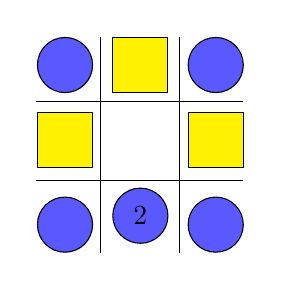
\begin{tikzpicture}
\matrix (m) [matrix of nodes, style grid={draw}, nodes in empty cells, label skeleton, row sep=2mm, column sep=2mm, nodes={minimum size = 0.8cm}] {
 \bl{} & \wh    & \bl{} \\ 
 \wh   &        & \wh   \\ 
 \bl{} & \bl{2} & \bl{} \\
};
\end{tikzpicture}
\end{center}
\caption{An example game state after the first move of the blue player on a $3\times 3$ board.
The center brick was moved down, creating a tower of height 2 with a blue top brick and a yellow brick below (not shown here).
The board's center will now remain empty for the rest of the game.
Moving the center tower is the optimal choice; due to symmetries, any direction is equally good, leading to a win for blue by a margin of 3.
If the yellow player started, they could win by a margin of 1 (game value -1) by first taking over the board's center.
} \label{fig:example-state}
\end{figure}
As already mentioned, the game can be played on rectangular boards of arbitrary sizes.
This makes it difficult to apply size-specific optimizations like bitboards.
However, independent of its shape, the game board is symmetrical along both axes.
This means that on a $3\times3$ board, say, moving the center tower up or down in the first turn yields equivalent game states (Fig. \ref{fig:example-state}).
In addition, square boards are rotationally symmetrical, that is on this particular board, moving the center tower left or right also yields states equivalent to the ones mentioned before.
So far, openings have not been studied deeply, and no best first move has been discovered for arbitrary board shapes.
Therefore, exploiting the symmetries is the main tool for reducing the number of moves to consider in the first turns.
They allow to ignore roughly half the moves on average.
On square boards and boards with only odd side lengths, another factor of ca. $0.5$ can be ignored, respectively.
The proof and exact numbers are not provided here, however, as they are too verbose for this paper.
Moreover, by exploiting symmetries it is possible to build and store tables of interesting positions more effectively.

\paragraph{Isolation}
The game rules state that towers can only be placed on top of other towers.
In particular, they must not be moved to fields that are already empty.
Several consequences follow from this.
First, the number of towers is an upper bound for the overall number of moves in a game as with each move the number of towers on the board must decrease by one (the number of towers $-1$ to be precise, as there is no legal move with only one tower on the board).
Although the number of moves in a game is usually somewhat lower (on average 72\% of the maximum, although the number is higher if both players are good \cite{Althöfer2020}) this can possibly be used for time management to estimate the remaining length of a game.
Second, if a player at some point has no legal move left, they have to skip.
In this situation it is clear that none of their towers has an adjacent tower, otherwise skipping is not allowed.
It follows that also in the future progression of the game, none of the skipping player's towers will be able to move.
At this point, the evaluation module does not have to search a game tree anymore, but only count the maximum height reachable for the player that is still active.
Third, as the game progresses the board gets sparse.
Analogously to matrices, it might be beneficial to use a representation different from an array in that case.
While this likely plays a minor part for smaller boards, the effects on larger boards can be dramatic, especially in the end game where large portions of the board are free.
During move generation, all towers of the active player have to be iterated.
This operation is highly inefficient if, for instance, 70\% of all fields are empty.
Here, using a map to store the board (or possibly two maps: one for each player) should reduce the runtime considerably.
Towers that have no neighbors can easily be ignored during move generation as they will not be able to move ever again.
However, move generation is not the only computational cost.
The other part is the evaluation step.
For that, \emph{all} towers on the board must be iterated to consider their height.
Early on, this process is perfectly efficient using an array representation, allowing vectorized processing.
Small boards, moreover, fit completely into a single cache line in that model.
Altogether, it is expected that there is some turn number (dependent on the board \emph{shape}) at which it is beneficial to change the board representation from an array to a map.
(The word \emph{shape} is used instead of \emph{size} to emphasize that computations on a $1\times15$ board are much easier than on a $3\times5$ board, although the number of fields is equal \cite{Althöfer2020}.)
As this number is probably also dependent on the hardware being used (e.g. the vector instruction set), it is suggested to leave this up to the user's choice via a parameter.
The evaluation step also carries room for minor optimizations in a map representation similar to the ones mentioned above at the generation phase.
Isolated towers may be immovable, but they are also \emph{safe}:
the opponent can not take them over, so they form an upper bound for the margin a player can loose by.
This means that only a single isolated tower with the maximum height for each player has to be stored as all others won't affect the outcome.
The towers on the board tend to decay into many isolated regions in the end game.
This behavior is well known from the related game Clobber \cite{Althöfer2004}.
Therefore, ignoring a large portion of irrelevant towers in the end game allows the evaluation module to find the truly important towers in the current state.
This technique only works for single isolated towers, though.
It is not possible to ignore whole regions of connected towers whose sum of heights is lower than the height of some other isolated tower.
As soon as towers are connected, they can be moves which means that they contribute to maneuvers like zugzwang in other regions on the board.
This can be ignored, of course, if some player has a safe tower that is higher than any other active region can sum up to, but this happens fairly rarely if both players are about equally strong.

% TODO find a good headline
\paragraph{Board value caching}
The next optimization is based on observing when the game value changes.
As it is only based on the highest towers, it is inherently robust to most changes on the board.
Hence, much computation can be saved when the height of the highest towers for each player is cached.
It only has to be updated in two cases:
First, a player creates a new highest tower.
In that case, the cached number just has to be overwritten which is a cheap operation.
Second, the opponent takes over a tower with the same height as the cached maximum.
This is the only (comparatively) expensive case as the whole board must be searched to find the new highest tower.
The cache can be extended to the top $k$ towers for each player to delay the full search case.
It is open for which $k$ the cache management becomes too costly to be effective (remember that the first case creates linear overhead for $k$ cached heights).

\subsection{High-level considerations}
\paragraph{Search algorithm}
Searching game trees typically comes in two flavors:
\enquote{full} search and Monte Carlo search (or a combination thereof).
The former searches every possible game state that is reachable from the current state, and returns a path that leads to the best outcome for the active player.
It is most effective if the game state complexity is manageable.
Otherwise, this method may not find the best (or even a good) move within acceptable time.
It is required to use this method, if exact game values are needed, e.g. in theoretical analysis of the game.
In practical settings, some form of $\alpha$-$\beta$-pruning is always applied as it cuts off branches of the search tree that will not influence the outcome.
For the pruning to work most effectively, the best move has to be searched first.
This leads to a chicken-and-egg problem that is typically solved by using a heuristic for the move ordering as discussed in the next paragraph.

Monte Carlo tree search (MCTS) is applied in settings where there are too many states to search completely (or even pruned).
Its core idea is to consider random moves, collect statistics about their outcomes, and choose the move that has the highest probability of being good.

In San Jego, the game state space becomes unmanageable quite early.
\citeauthor{Althöfer2020} report that the full search on boards as small as $5\times5$ with their NegaScout implementation (an optimized version of $\alpha$-$\beta$-pruning) took \enquote{several days} \cite[p.~8]{Althöfer2020}.
Using the optimizations outlined in section \ref{subsec:low-level}, it is likely possible to bring that number down.
Typical computer olympiad matches of similar games, however, are played on $10\times10$ boards \cite{Wojciech2011}, which is completely hopeless to encounter with full search.
Therefore, MCTS should be used for San Jego playing programs.
One important property here is that the branching factor monotonically decreases in the course of the game, as each turn a tower is effectively eliminated.
This makes full tree search applicable in the end game to play that phase more precisely.

Game tree search, either full or stochastical, can usually be parallelized easily.
Several units, be it threads, processes or even machines, can search different subtrees of the present game state concurrently.
In naive implementations using a static scheduling, however, concurrent units can starve quickly, and become useless as soon as it becomes apparent that their subtree can be cut off while pruning.
Hence, evaluation of states should be implemented using tasking or iterative deepening.


\paragraph{Search strategy}
An important factor for the success of game tree searching is the evaluation function.
In some combinatorial games like chess and Go, the value of a game state is generally not known.
Other games, as San Jego, define a value for each game state, but it might not be good approach for sorting candidate moves.
For instance, consider the first turn in a game.
Whatever move the player chooses, they all lead to a game state with the same value of $+1$.
Therefore, several improvements are possible.
\citeauthor{Althöfer2020} found that a combination of prioritizing moves that target high enemy towers and deprioritizing moves that target high own towers on the one hand, and prioritizing moves targetting the center of the board on the other hand work together nicely.

In a concurrent setting, some of the units can also be used to run more complex analyses on the game state.
In San Jego, this could include analysis of the isolated regions to find optimal moves to solve them.
Although it was already lined out that these regions can not simply be evaluated independently from each other due to effects as zugzwang, this analysis can help to find critical moves to aid in move ordering.
Regions are harder to evaluate the more \enquote{rectangular-like} they are as the branching factor gets bigger.
In practice, the rectangular regions with the shape $3\times4$ can be evaluated within few seconds even by a simple, single-threaded python program that does not use any of the optimizations laid out in the previous subsection, giving an idea for the size of regions feasible for this kind of analysis.

%\begin{itemize}
  %\item board is symmetrical and rotationally invariant -> speed up start
  %\item towers can not move to empty fields -> each turn a tower is removed -> max number of turns is fixed and depends on board size
  %\item what move to choose in first turn? all moves produce same board value -> empirically: moves to center of boards are more powerful on average \cite{Althöfer2020}
  %\item max tower height: m*n => can be used for representation improvement
  %\item cache the hights of the highest towers of both players (avoids costly recalculation in every explored node); recalculation only necessary if new higher tower was built or a tower with the max height of a player was taken
  %\item if a player had to skip once, there will never be a move available to them again
  %\item isolated regions
%\end{itemize}

\section{Implementation}
Additionally to the theoretical analysis, this paper provides a San Jego library implementation.
It can be used in the future to test different bot implementations and optimizations against a baseline.

The library itself is written in C++ and managed by the CMake build system.
It makes use of templates to describe board sizes.
This way, compile-time optimizations are available such as the bits for the tower data structure as outlined in subsection \ref{subsec:low-level}. 
For simplicity, and in order to not disturb alignment of the underlying integers, a whole byte is used to back the towers.
It is sufficient to play on board with up to 127 fields, which includes the \enquote{olympic} size of $10\times10$.
As towers can not have a height of 0, this representation is used for absent towers on the board.

The board itself is represented as a vector of towers (an array of bytes, eventually) which makes it very memory-efficient and thus cache-friendly.
It provides operations to make and undo moves, to retrieve towers, and to find the the towers of maximum height for each player.
The loop to compute this latter value is not easily auto-vectorizable as it contains jumps that depend on the top brick color of each tower.
However, if it turns out that this computation still uses a great share of computation time after the above mentioned caching of height values was applied, the condition on the color could be replaced by a multiplication of the tower height with the boolean \texttt{tower.top()==color\_of\_interest} which is implicitly converted to $0$ or $1$ (C++ standard \texttt{\S4.5/4}).
Note that the board itself has not included any game logic in the sense of rules.
Any move can be applied, except for moves that target fields outside the underlying vector's bounds.

The rule set is implemented independently in its own header file.
This decoupling makes it possible to reuse the board for different rule sets, or a rule set for different board implementations.
Rules stem from an abstract base class, and must implement a method that decides whether a move is legal or not, and a method to evaluate a game state.
Other operations as iterating all legal moves, or determining whether the game has ended follow from these to rules, but are implemented explicitly which allows for further optimizations and clarity.

Lastly, the library defines an abstract explorer class that encapsulates the game tree search.
It takes a rule set as a parameter to make it reusable for many rule sets.
This standard implementation only defines a weak dummy bot that looks one move ahead, but more sophisticated explorers can be added easily.

Great emphasis was placed on correctness when implementing the standard library, hence it comes with a couple of test cases described using the Catch2 unit test library.
Future optimizing steps can rely on them to ensure they do not break things.

The library is published under the MIT license, and is tested with gcc, clang and MSVC under GNU/Linux and Windows.

\section{Conclusions}
The game of San Jego is a great playground to implement and test efficient and clever algorithms on.
This paper makes many suggestions as to what techniques a playing program could (and probably should) be using in order to achieve the best results possible today.
It also provides an correct, efficient and well-organized standard library implementation that will boost the development of San Jego bots in the future.

\bibliographystyle{ACM-Reference-Format}
\bibliography{literature}


\end{document}
\endinput
